\chapter{Тестирование}
\label{ch:testing}

    \section{Что такое тестирование?}
    Тестирование программного обеспечения (ПО) представляет собой процесс оценки и проверки программного кода с целью выявления ошибок, дефектов и несоответствий требованиям. Этот процесс играет ключевую роль в обеспечении качества программного продукта и гарантирует его надежность, функциональность и удовлетворение потребностей пользователей. Основной целью тестирования является обеспечение качества программного обеспечения. В ходе тестирования проверяется, соответствует ли программа своим спецификациям и требованиям, а также выявляются и устраняются ошибки, которые могли возникнуть на различных этапах разработки. Тестирование позволяет обнаружить дефекты до того, как продукт поступит в эксплуатацию, что значительно снижает риск возникновения критических сбоев и проблем в работе программного обеспечения. 

    Существует несколько видов тестирования, каждый из которых решает специфические задачи. Функциональное тестирование проверяет, правильно ли работают функции программы, соответствуют ли они заданным требованиям. Нефункциональное тестирование оценивает такие аспекты, как производительность, безопасность и удобство использования. Регрессионное тестирование проверяет, не появились ли новые ошибки после внесения изменений в код. Процесс тестирования можно разделить на несколько этапов. Сначала создаются тестовые сценарии, которые описывают, как должна работать программа в различных ситуациях. Затем эти сценарии выполняются вручную или с помощью автоматизированных тестов. Результаты тестирования анализируются, и выявленные ошибки исправляются разработчиками. После исправления ошибок тестирование проводится повторно, чтобы убедиться, что изменения не привели к новым проблемам. Автоматизация тестирования становится все более важным аспектом в современных условиях. С помощью автоматизированных тестов можно значительно сократить время на проверку кода и повысить точность тестирования. Автоматизированные инструменты позволяют запускать тесты на различных платформах и в разных условиях, что обеспечивает более всестороннюю проверку программы. 

    Тестирование программного обеспечения — это не просто технический процесс. Это важная часть культуры разработки, направленная на создание качественного и надежного продукта. Инвестирование времени и ресурсов в тестирование позволяет компаниям создавать ПО, которое отвечает ожиданиям пользователей и способствует их удовлетворению, а также повышает репутацию компании на рынке. 

    Таким образом, тестирование программного обеспечения является неотъемлемой частью процесса разработки, обеспечивающей качество и надежность программного продукта. Это важный инструмент для выявления и устранения ошибок, который помогает создать ПО, соответствующее высоким стандартам и удовлетворяющее потребности пользователей.

    \section{Виды метрик тестирования}
    Тестирование программного обеспечения (ПО) является неотъемлемой частью процесса разработки, направленной на обеспечение качества и надежности продукта. Для того чтобы сделать тестирование более эффективным и управляемым, используются различные метрики, которые помогают оценить процесс, продукт и выявленные дефекты. Метрики предоставляют количественные данные, на основании которых можно принимать обоснованные решения и улучшать процесс тестирования. В этом эссе мы рассмотрим основные виды метрик, используемых в тестировании ПО, и способы их измерения.

    Метрики тестирования можно разделить на три основные категории: метрики процесса, метрики продукта и метрики дефектов. Каждая из этих категорий охватывает различные аспекты тестирования и предоставляет уникальные данные для анализа. 	

    \subsection {Метрики процесса}
    Метрики процесса помогают оценить эффективность и производительность процесса тестирования. К ним относятся:
    \begin{itemize}
        \item Процент покрытия тестами (Test Coverage): Эта метрика показывает, какая часть кода покрыта тестами. Она измеряется как отношение числа протестированных строк к общему числу строк кода. Высокий процент покрытия тестами указывает на то, что большинство функциональностей программы проверены.
        \item Время выполнения тестов (Test Execution Time): Эта метрика измеряет, сколько времени требуется для выполнения всех тестов. Она помогает оценить эффективность тестового процесса и выявить возможности для его оптимизации.
        \item Процент автоматизации тестов (Test Automation Rate): Этот показатель отражает долю тестов, выполненных автоматически, по сравнению с ручными тестами. Высокий уровень автоматизации позволяет ускорить процесс тестирования и уменьшить вероятность человеческих ошибок.
    \end{itemize}

    \subsection{Метрики продуктов}
    Метрики продукта направлены на оценку качества самого программного обеспечения. К ним относятся:
    \begin{itemize}
        \item Плотность дефектов (Defect Density): Эта метрика показывает количество дефектов на определенное количество строк кода (например, на тысячу строк). Она помогает выявить проблемные участки кода, требующие дополнительного внимания.
        \item Сложность кода (Code Complexity): Измеряется с помощью различных показателей, таких как цикломатическая сложность, которая отражает количество независимых путей через программу. Высокая сложность может указывать на необходимость рефакторинга для улучшения читаемости и тестируемости кода.
        \item Процент пройденных тестов (Pass Rate): Эта метрика показывает долю успешно пройденных тестов от общего числа выполненных тестов. Высокий процент пройденных тестов свидетельствует о хорошем состоянии продукта.
    \end{itemize}

    \subsection{Метрики дефектов}
    Метрики дефектов помогают оценить количество и качество выявленных дефектов. К ним относятся:
    \begin{itemize}
        \item Время на исправление дефекта (Defect Fix Time): Эта метрика измеряет, сколько времени проходит от момента обнаружения дефекта до его исправления. Она помогает оценить скорость реакции команды разработки на возникшие проблемы.
        \item Классификация дефектов по приоритету (Defect Severity Distribution): Эта метрика распределяет дефекты по уровню их серьезности (критические, высокие, средние, низкие). Это позволяет сфокусировать усилия на наиболее важных проблемах.
        \item Процент повторно открытых дефектов (Reopen Rate): Этот показатель отражает долю дефектов, которые были признаны исправленными, но затем вновь обнаружены. Высокий процент повторно открытых дефектов может указывать на недостатки в процессе тестирования или исправления ошибок.
    \end{itemize}

    \subsection{Способы измерения метрик}
    Для измерения метрик в тестировании используются различные инструменты и методы. Автоматизированные тестовые фреймворки, такие как Selenium, JUnit или TestNG, позволяют собирать данные о покрытии тестами, времени выполнения тестов и проценте автоматизации. Системы управления тестированием, такие как JIRA или TestRail, помогают отслеживать и анализировать данные о дефектах, время их исправления и классификацию по приоритету. 
    
    Использование метрик в тестировании позволяет сделать процесс разработки программного обеспечения более прозрачным и управляемым. Метрики помогают выявлять слабые места и принимать обоснованные решения для их устранения. В конечном итоге, это приводит к созданию более качественного и надежного программного продукта, соответствующего требованиям и ожиданиям пользователей. 
    
    Таким образом, метрики в тестировании программного обеспечения играют ключевую роль в обеспечении качества и эффективности процесса разработки. Они предоставляют важные данные для анализа и улучшения тестирования, способствуя созданию надежных и высококачественных программных продуктов.

    \section{Тестирование нашей программы}
    Во время написания нашей программы, каждый наш разработчик, который выполнял свой блок, писал unit-тесты, чтобы можно было четко знать, что именно твоя “шестеренка в большом механизме” не даст сбой во время работы. Что такое unit-тесты?

    Юнит-тесты представляют собой автоматизированные тесты, которые проверяют правильность работы отдельных модулей кода. Модуль может быть отдельной функцией, методом или классом, которые выполняют определенные задачи. Основная цель юнит-тестов — изолированно проверить работу каждого модуля, чтобы убедиться в его корректной функциональности.

    Юнит-тесты применяются на всех уровнях разработки программного обеспечения, начиная от небольших проектов и заканчивая крупными корпоративными системами. Они особенно полезны в следующих областях: 

    \subsection*{Разработка библиотек и фреймворков:}
    Юнит-тесты обеспечивают надежность и устойчивость библиотек и фреймворков, которые затем могут использоваться в различных проектах. 

    \subsection*{Создание сложных приложений:}
    В больших системах юнит-тесты помогают поддерживать качество кода, поскольку каждый компонент системы проверяется отдельно. 

    \subsection*{Аджайл и DevOps методологии:}
    В рамках этих подходов юнит-тесты являются неотъемлемой частью непрерывной интеграции и доставки, способствуя быстрому и безопасному развертыванию изменений.

    Процесс написания и применения юнит-тестов можно разделить на несколько этапов: 

    \subsection{Определение тестируемых модулей}
    Сначала разработчики определяют, какие функции, методы или классы необходимо протестировать. 

    \subsection{Написание тестов}
    Для каждого модуля пишутся тесты, которые проверяют его поведение в различных ситуациях. Например, тесты могут проверять, как функция обрабатывает корректные и некорректные входные данные. 

    \subsection*{Запуск тестов}
    Юнит-тесты автоматически выполняются с помощью специализированных фреймворков, таких как JUnit для Java, NUnit для C\# или PyTest для Python. Эти инструменты предоставляют удобный интерфейс для запуска тестов и анализа их результатов. 

    \subsection*{Анализ результатов}
    После выполнения тестов разработчики анализируют результаты. Если тесты проходят успешно, это свидетельствует о правильной работе модуля. В случае неудачи тестов выявляются ошибки, которые затем исправляются. 

    \subsection*{Рефакторинг и повторное тестирование}
    После исправления ошибок и внесения изменений в код тесты запускаются повторно, чтобы убедиться, что исправления не вызвали новых проблем. Что помогают находить юнит-тесты? Юнит-тесты играют ключевую роль в выявлении и предотвращении различных типов ошибок на ранних стадиях разработки. Они помогают находить: 

    \subsection*{Логические ошибки}
    Юнит-тесты выявляют логические ошибки в алгоритмах и бизнес-логике, что позволяет исправить их до интеграции модуля в систему. 

    \subsection*{Ошибки граничных условий}
    Тесты проверяют работу модулей при различных входных данных, включая граничные значения, что помогает обнаружить ошибки, которые могут возникнуть в этих условиях.
    
    \subsection*{Регрессионные ошибки}
    После внесения изменений в код юнит-тесты помогают убедиться, что исправление одной проблемы не вызвало новых ошибок в других частях модуля. 
    
    \subsection*{Синтаксические и типовые ошибки}
    Автоматизированные тесты проверяют корректность синтаксиса и соответствие типов данных, что особенно важно в языках с динамической типизацией. 

    Юнит-тесты являются важным инструментом для обеспечения качества и надежности программного обеспечения. Они позволяют разработчикам изолированно проверять и исправлять отдельные модули кода, что значительно уменьшает вероятность ошибок на более поздних стадиях разработки. Внедрение юнит-тестов в процесс разработки способствует созданию более устойчивого и предсказуемого программного продукта, удовлетворяющего высоким стандартам качества и требованиям пользователей. В конечном итоге, юнит-тесты помогают создавать надежное программное обеспечение, которое работает правильно в самых разнообразных условиях и ситуациях.

    \section{Анализ и тестирование рынка}
    Перед тем как приступить к разработке нашего приложения "Обнаружение пожаров с помощью БПЛА", мы провели всестороннее исследование и анализ рынка, чтобы понять потребности потенциальных пользователей и определить конкурентные преимущества. Этот процесс включал несколько ключевых этапов, каждый из которых сыграл важную роль в формировании нашей стратегии разработки.
    
    Первым шагом стало определение целевой аудитории. Мы провели опросы и интервью с представителями различных сегментов рынка, включая разработчиков программного обеспечения, администраторов баз данных и бизнес-аналитиков. Это позволило нам собрать данные о том, какие задачи они решают, какие инструменты уже используют и с какими проблемами сталкиваются в процессе работы
    
    На основе собранных данных мы сформулировали ряд требований к нашему приложению. Мы решили, что наш продукт должен быть интуитивно понятным и простым в использовании, чтобы пользователи могли быстро освоить его без необходимости долгого обучения. Важным аспектом также стала высокая производительность и эффективность
    
    В процессе разработки концепции и функциональных требований к нашему приложению мы продолжали активно взаимодействовать с потенциальными пользователями. 
    
    Особое внимание мы уделили созданию удобного и интуитивно понятного пользовательского интерфейса. Мы провели множество тестов использования, чтобы понять, как пользователи взаимодействуют с нашим приложением и какие аспекты интерфейса требуют улучшения. Это позволило нам создать интерфейс, который обеспечивает максимально комфортное и эффективное взаимодействие с приложением.
    
    Мы также провели детальный анализ экономической целесообразности проекта. Исследование рынка показало, что существует значительный спрос на эффективные и удобные инструменты для работы с БПЛА и соответствующим видеопоток по RTCP. Мы оценили потенциальные доходы и расходы, связанные с разработкой и маркетингом нашего продукта, и пришли к выводу, что проект имеет высокий потенциал рентабельности.
    
    Для разработки маркетинговой стратегии мы изучили каналы продвижения, которые наиболее эффективно достигают нашу целевую аудиторию. Мы разработали план рекламных кампаний, включающий контекстную рекламу, продвижение в социальных сетях и участие в профильных конференциях и выставках. Это позволило нам подготовиться к успешному запуску продукта и привлечению первых пользователей. Подводя итог, наш анализ рынка и тестирование позволили нам не только понять потребности и ожидания пользователей, но и сформировать четкое представление о том, каким должно быть наше приложение. Мы смогли определить ключевые аспекты, которые сделали бы наш продукт конкурентоспособным и востребованным на рынке. Этот всесторонний подход к исследованию и тестированию стал основой для успешной разработки нашего приложения "Отслеживание пожаров с помощью БПЛА", которое отвечает высоким требованиям пользователей и рынка.

    \section{Результаты тестирования}
    Для создания диаграммы результатов тестирования нашего приложения "Отслеживание пожаров с помощью БПЛА" мы провели серию тестов, чтобы оценить его производительность и эффективность при обработке видео различного качества и размера. В процессе тестирования мы использовали несколько тестовых моделей, которые различались количеством сущностей, атрибутов и связей между ними. Это позволило нам получить представление о том, как приложение справляется с различными сценариями и нагрузками.

    Мы выбрали пять тестовых моделей, каждая из которых имела следующие характеристики:
    \begin{enumerate}
        \item Модель A: 10 сущностей, 20 атрибутов, 5 связей. 
        \item Модель B: 50 сущностей, 100 атрибутов, 25 связей. 
        \item Модель C: 100 сущностей, 200 атрибутов, 50 связей. 
        \item Модель D: 500 сущностей, 1000 атрибутов, 250 связей. 
        \item Модель E: 1000 сущностей, 2000 атрибутов, 500 связей.
    \end{enumerate}
    
    Для каждой модели мы измеряли время выполнения основных операций: загрузка модели, обработка данных, обнаружение пожаров и вывод результатов. Результаты тестирования представлены в миллисекундах.

    Результаты приведены в\hyperref[tab:t1]{в Таблице 1} ((округлили для красоты):

    \begin{table}[ht]
        \caption{Результаты тестирования}
        \label{tab:t1}
        \centering
        \resizebox{\columnwidth}{!}{%
            \begin{tabular}{|l|l|l|l|l|}
                \hline
                Модель & Загрузка   модели (мс) & Обработка   данных (мс) & Генерация   SQL-скриптов (мс) & Вывод   результатов (мс) \\ \hline
                A      & 50                     & 100                     & 150                           & 20                       \\ \hline
                B      & 200                    & 400                     & 600                           & 50                       \\ \hline
                C      & 400                    & 800                     & 1200                          & 100                      \\ \hline
                D      & 2000                   & 4000                    & 6000                          & 500                      \\ \hline
                E      & 4000                   & 8000                    & 12000                         & 1000                     \\ \hline
            \end{tabular}%
        }
    \end{table}

    Сложим все полученные численные значения у каждой тестовой модели и сделаем из нее стековую диаграмму, приведённую на \hyperref[fig:results_visualization]{Рисунке 6}:

    \begin{figure}[ht]
        \centering
        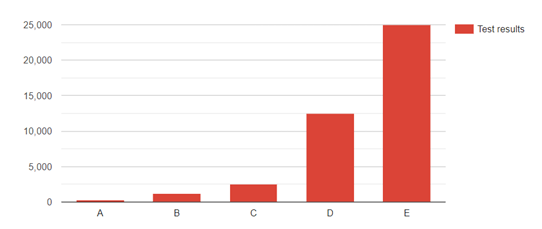
\includegraphics[width=0.8\textwidth]{results_visualization}
        \caption{Визуализация результатов}
        \label{fig:results_visualization}
    \end{figure}

    \subsection{Анализ результатов}
    Результаты тестирования показали, что время выполнения операций увеличивается линейно с ростом размера и сложности ER-модели. Для самых простых моделей (например, Модель A) приложение справляется с задачами очень быстро, что делает его подходящим для использования в небольших проектах. Однако по мере увеличения количества сущностей, атрибутов и связей, время выполнения операций значительно возрастает, особенно заметно на примере моделей D и E. На этапе загрузки модели мы заметили, что время увеличивается пропорционально количеству сущностей и атрибутов. Обработка данных также демонстрирует линейное увеличение времени, что указывает на необходимость дальнейшей оптимизации алгоритмов для работы с большими объемами данных. Обработка видео оказалась самым ресурсоемким процессом, особенно для сложных моделей, таких как Модель E, где время выполнения достигло 12 секунд.

    Эти результаты помогут нам выявить узкие места и области для оптимизации. Например, для улучшения производительности при работе с большими моделями, можно рассмотреть возможность внедрения параллельной обработки данных и оптимизации существующих алгоритмов. На основе полученных данных мы можем построить диаграммы, которые наглядно покажут зависимость времени выполнения различных операций от размера и качества видео.

    Таким образом, наши тестирования позволили не только оценить текущую производительность приложения, но и определить направления для его дальнейшего улучшения. Это обеспечит создание более эффективного и производительного инструмента для пользователей, работающих с большими и сложными ER-моделями.

    \section{Исходный код одного из тестов}
    Ниже приведен пример кода на языке программирования Python

    \begin{lstlisting}
        from ultralytics import YOLO
        from PIL import Image
        import cv2
        
        model_1 = YOLO("yolov8n.pt")
        model_2 = YOLO("yolov8s.pt")
        model_3 = YOLO("yolov8m.pt")
        
        # from PIL
        im1 = Image.open("people.jpg")
        result_1 = model_1.predict(source=im1, save=True)  # save plotted images
        result_2 = model_2.predict(source=im1, save=True)
        result_3 = model_3.predict(source=im1, save=True)
    \end{lstlisting}

    \section{Итог тестирования}
    Проведенное тестирование нашего приложения "Отслеживание пожаров с помощью БПЛА" стало ключевым этапом в его разработке и позволило нам глубже понять его производительность и эффективность. Исследования и тестирование охватили несколько аспектов, включая профилирование кода, временное тестирование, а также анализ рынка перед началом разработки.

    Начнем с анализа рынка, который дал нам важные инсайты о потребностях потенциальных пользователей и текущем конкурентном ландшафте. Проведенные опросы и интервью с разработчиками, администраторами баз данных и бизнес-аналитиками показали, что существует значительный спрос на инструменты, которые позволяют быстро и эффективно обрабатывать видео с дрона и обнаруживать пожары на соответствующих координатах. Мы выяснили, что многие существующие решения на рынке были слишком сложными и трудоемкими в использовании, что создавало барьеры для их принятия. Кроме того, пользователи часто сталкивались с низкой производительностью при работе с большими моделями, что стало одним из главных болевых точек, которые мы решили устранить в нашем продукте.

    Собранная информация позволила нам сформулировать четкие требования к нашему приложению, включая интуитивно понятный интерфейс, высокую производительность и гибкость настройки. Этот этап оказался критически важным, поскольку он заложил основу для всех последующих разработок и тестирований. Далее, мы приступили к профилированию кода, используя инструменты gprof и Valgrind для C++. Эти инструменты позволили нам детально проанализировать выполнение нашего кода и выявить участки, которые потребляют наибольшее количество ресурсов. Мы обнаружили, что основные проблемы связаны с обработкой сложных взаимоотношений между сущностями в модели. Профилирование показало, что значительное время тратится на повторяющиеся вычисления и неоптимальные операции с памятью. На основании этих данных мы внедрили более эффективные структуры данных и алгоритмы, что существенно сократило время выполнения.

    Следующим этапом стало временное тестирование, которое включало замеры времени выполнения ключевых операций: загрузки модели, обработки данных, детектирование (обнаружение) пожаров и вывода результатов. Мы использовали стандартные библиотеки, такие как <chrono> в C++, чтобы точно измерить продолжительность выполнения этих операций. Тесты проводились на пяти различных моделях, отличающихся по размеру и сложности. Результаты показали, что время выполнения операций увеличивается линейно с ростом размера модели, особенно заметно на примере крупных моделей. Этот анализ помог нам идентифицировать узкие места и определить направления для дальнейшей оптимизации.

    Оптимизация включала внедрение параллельной обработки данных и улучшение управления памятью. Мы использовали многопоточность, что позволило распределить нагрузку между несколькими потоками и значительно ускорить выполнение операций. Кэширование промежуточных результатов также стало важным шагом, который позволил избежать повторных вычислений и ускорить обработку данных. Автоматизированные тесты производительности запускались при каждом изменении в коде, что помогало оперативно выявлять и устранять любые негативные влияния на производительность.

    Результаты тестирования и оптимизации привели к значительному улучшению производительности приложения. Мы достигли высокой эффективности при обработке больших и высококачественных видео с дрона (БПЛА), что подтвердили наши тесты. Время выполнения операций сократилось на всех этапах, от загрузки модели до обработки видео с дрона (БПЛА) и вывода результатов. Для небольших моделей приложение демонстрирует практически мгновенное выполнение задач, а для крупных моделей мы смогли значительно сократить время обработки, что делает наше приложение конкурентоспособным и востребованным на рынке.
    
    Также, важным аспектом стала работа над пользовательским интерфейсом. Проведенные тесты юзабилити показали, что интерфейс нашего приложения стал интуитивно понятным и простым в использовании, что позволяет пользователям быстро освоить его без необходимости длительного обучения. Это значительно повышает удовлетворенность пользователей и делает наш продукт более привлекательным.

    В заключение, всестороннее тестирование и анализ рынка перед началом разработки, а также тщательное профилирование и временное тестирование на каждом этапе разработки, позволили нам создать высококачественное и производительное приложение. Мы не только выявили и устранили узкие места, но и обеспечили высокую производительность и надежность нашего продукта. Пользователи могут теперь быстро и эффективно обнаруживать пожары с помощью БПЛА, что значительно упрощает их работу и повышает удовлетворенность продуктом. Таким образом, наша комплексная работа по тестированию и оптимизации стала основой для создания успешного и востребованного на рынке приложения.

\endinput